%!TEX root = ../../../report.tex

\section{Geometrical dimensions of the frame} % (fold)
\label{sec:dimensions}

The selection of the final dimensions of RuBi corresponds to an iterative process in which power requirements have been the first constraint when assessing the size of the robot.
A first approach was taken from \cite{grimmer}, Manuscript I, where normalized values of power required per joint and per kilogram of weigh of the structure can be found.
The first iteration targeted a robot of dimensions $m = 1Kg$ and length from the hip joint to the toes of $L = 0.6 m$.
The final parameters from the last iteration can be found in %***chapter Results

Once estimated an overall height of the structure, the dimensions of each link were decided to be obtained from the German table of the ISO 7250-2 \cite{iso_measurements} and the DIN 33402-2 \cite{din_measurements1} norms, following the idea of mimicking human-like motion as closely as possible.
These two norms are standard references in industry and were considered a general enough source of information.
Figure \ref{fig:human_measurements} depicts the human dimensions extracted from the norms and applied to the design of RuBi.

\begin{figure}[h]
	\centering
	\begin{subfigure}[b]{0.3\textwidth}
        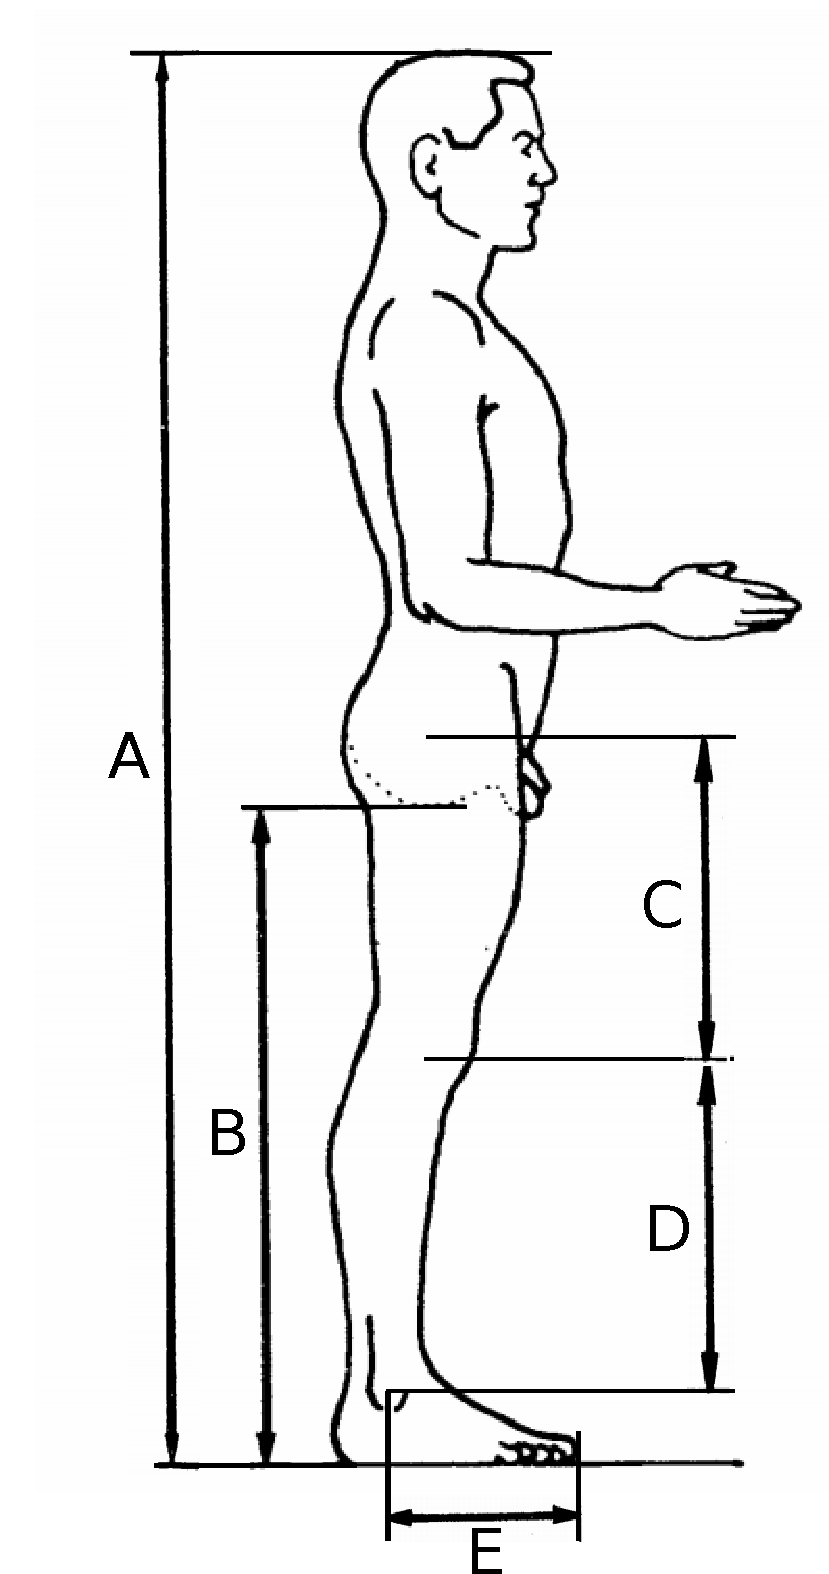
\includegraphics[width=\textwidth]{figures/din_measurements.pdf}
        \caption{Left foot}
        \label{fig:din1}
    \end{subfigure}
    \begin{subfigure}[b]{0.4\textwidth}
        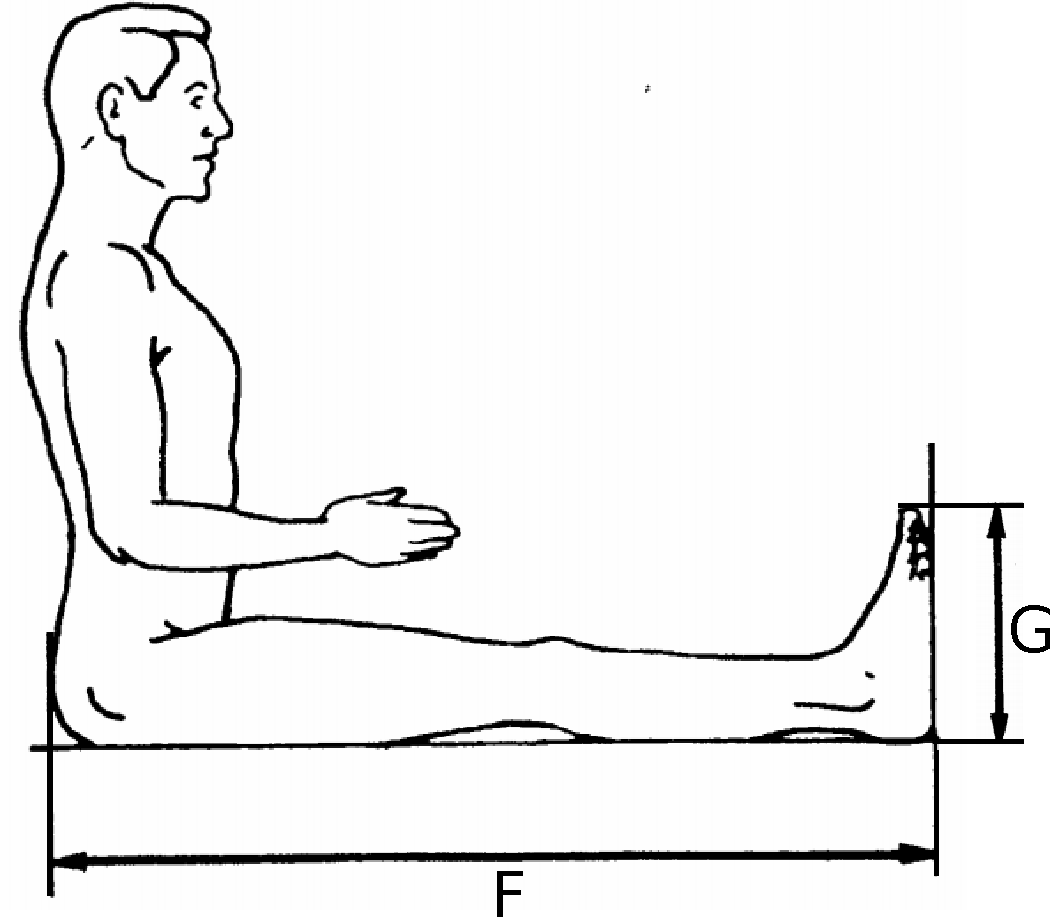
\includegraphics[width=\textwidth]{figures/din_measurements2.pdf}
        \caption{Hip}
        \label{fig:din2}
    \end{subfigure}
	\caption{Lower body measurements used for RuBi. Picture adapted from \cite{din_measurements1}.}
	\label{fig:human_measurements}
\end{figure}

The crotch height, denoted as $B$ in the figure, has been matched to the distance from the hip joint to the heel bottom in the robot 

\begin{table}
\begin{center}
	\begin{tabular}{c | c | c | c}
	  Index & Definition & Value & \% of Stature \\
	  \hline
	  A & Stature (body height) & 7 & 100 \\
	  B & Crotch height & 11 & \\
	  C & Femur height & 19 & \\
	  D & Tibial height & & \\
	  E & Ankle-toe tip distance & 5 & \\
	  F & Buttocks-leg length & & \\
	  G & Sole length & & 
	\end{tabular}
	\caption{Human proportions from DIN 33402-2}
	\label{tab:din_proportions}
\end{center}
\end{table}


%% Here we just describe the process followed to obtain the final dimensions. 
%% The final results are shown in Chapter Results --> add tables and Froude number calculus


% section dimensions (end)